\chapter{Implementation}

This chapter gives an overview of the implementation of the project.

% TODO: overview

\section{Repository Overview}

\begin{table}[H]
\centering
\begin{tabular}{lp{11cm}l}
\hline
\textbf{Directory} & \textbf{Description} & \textbf{LOC} \\
\hline
\texttt{core/} & Implementation of the core interpreter in Rust, including the parser, garbage collector, and the JavaScript FFI. & TBD \\
\texttt{core/src/wasm} & WebAssembly interface for the core interpreter and JavaScript FFI. & \\
\texttt{core/src/tests} & Unit tests for the core interpreter. & \\
\texttt{lib/} & Higher-level JavaScript library for the interpreter. & \\
\texttt{web/} & Web-based development environment to demonstrate and benchmark the interpreter. & \\
\texttt{web/src/prolog} & TypeScript Prolog interface and wrappers for various Prolog interpreters. & \\
\texttt{bench/} & Web-based benchmarking tools. & \\
\texttt{docs/} & Documentation for the project. & \\
\hline
\end{tabular}
\caption{An overview of key directories in the repository}
\label{tab:repository-overview}
\end{table}

\section{Core Interpreter}

This section describes the implementation of the core Prolog interpreter, implemented in Rust.

\subsection{Memory Layout}

\label{sec:memory-layout}

The interpreter uses the merged heap/stack architecture proposed by Li \cite{liEfficientMemoryManagement2000} and described in Section \ref{sec:preparation-implementation}. Alongside the advantages identified by Li, notably improved cache performance, this architecture is uniquely suited to the linear memory model of WebAssembly.

In a traditional heap/stack architecture, the heap and stack are separate regions of memory, often with few constraints imposed on the layout of the heap. Indeed, SWI-Prolog simply uses \texttt{malloc} to allocate memory for terms on the heap\footnote{\url{https://www.swi-prolog.org/pldoc/man?section=memlimit}}, imposing no constraints on where the C runtime decides to put the memory. Running natively, this is not a problem, as virtual memory is plentiful. However, WebAssembly's linear memory is contiguous and limited in size, so the heap must be carefully managed by the WebAssembly code itself to avoid fragmentation. In addition, the trail stack contains pointers to bound variables, which may appear either on the stack or on the heap, but WebAssembly does not allow pointers to exist to stack-allocated objects. Therefore, the stack must also be placed in the linear memory, which further complicates memory management.

In a merged heap/stack architecture, all terms are allocated in one contiguous region of memory. This avoids the problem of fragmentation, as the heap grows with allocations and shrinks with instant reclaiming and garbage collection (Section \ref{sec:gc-impl}). If the heap grows too large for the linear memory, it suffices, in theory, to execute the \texttt{memory.grow} WebAssembly instruction, with no additional work from the WebAssembly module required. In my implementation, the exact placement of the heap in the linear memory is decided by Rust's allocator, but once the heap grows sufficiently large, this has the same effect (Section \ref{sec:heap-placement}).

A key advantage of this architecture is that terms are stored in chronological order on the heap, with older terms at lower addresses. This facilitates the implementation of several garbage collection optimisations, such as variable shunting (Section \ref{sec:variable-shunting}) and generational stack collection (Section \ref{sec:generational-gc}).

Of course, other areas of memory are needed:

\paragraph{Trail Stack} The trail stack is a stack of pointers to variables that have been bound, used for backtracking.

\paragraph{Choice Point Stack} The choice point stack stores information about where to backtrack to for each choice we make. Alongside the next clause to consider, each choice point also contains the sizes of the heap, trail stack and goal stack to facilitate backtracking and instant reclaiming.

\paragraph{Goal Stack} The goal stack contains the remaining goals to prove. When backtracking, goals that have previously been popped might be needed again, so while I refer to it as a stack, the goal stack is actually a graph, with goals represented as pairs $(\texttt{pred}, \texttt{goal})$ and the goal stack additionally storing a pointer to the current goal (the ``top of the stack'').

\begin{figure}[H]
\centering
\begin{subfigure}{.5\textwidth}
\centering
\begin{minted}{prolog}
a(1).
a(2).
b(2).
?- a(X), b(X).

\end{minted}
\caption{A Prolog program}
\end{subfigure}%
\begin{subfigure}{.5\textwidth}
\centering
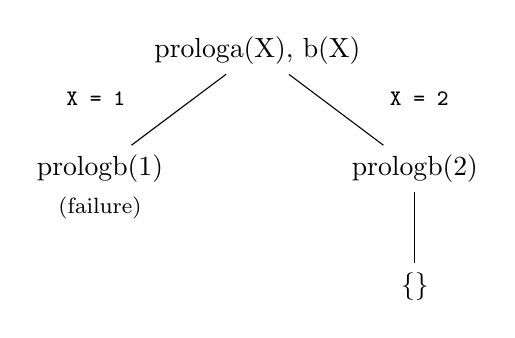
\begin{tikzpicture}
  \node (A) at (0,3) {\mintinline{prolog}{a(X), b(X)}};
  \node (B1) at (-2,1.5) {\mintinline{prolog}{b(1)}};
  \node (B2) at (2,1.5) {\mintinline{prolog}{b(2)}};
  \node (C2) at (2,0) {\{\}};

  \draw (A) -- (B1) node [midway, xshift=-30, yshift=4] {\footnotesize \texttt{X = 1}};
  \draw (A) -- (B2) node [midway, xshift=30, yshift=4] {\footnotesize \texttt{X = 2}};
  \draw (B2) -- (C2);

  \node (D) at (-2,1) {\footnotesize (failure)};
\end{tikzpicture}
\caption{Corresponding SLD-tree}
\end{subfigure}
\par\bigskip
\par\bigskip
\begin{subfigure}{.5\textwidth}
\centering
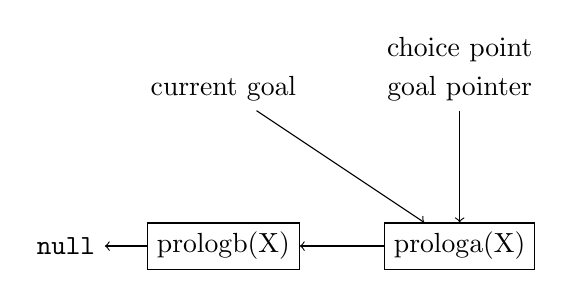
\begin{tikzpicture}[box/.style={draw, rectangle}]
  \node[box] (B) at (0, 0) {\mintinline{prolog}{b(X)}};
  \node[box] (A) at (3, 0) {\mintinline{prolog}{a(X)}};

  \node (null) at (-2, 0) {\texttt{null}};
  \node (current) at (0, 2) {current goal};
  \node (cp1) at (3, 2.5) {choice point};
  \node (cp2) at (3, 2) {goal pointer};

  \draw[->] (A) -- (B);
  \draw[->] (B) -- (null);
  \draw[->] (current) -- (A);
  \draw[->] (cp2) -- (A);
\end{tikzpicture}
\vspace{5mm}
\caption{The goal graph before the first resolution}
\end{subfigure}%
\begin{subfigure}{.5\textwidth}
\centering
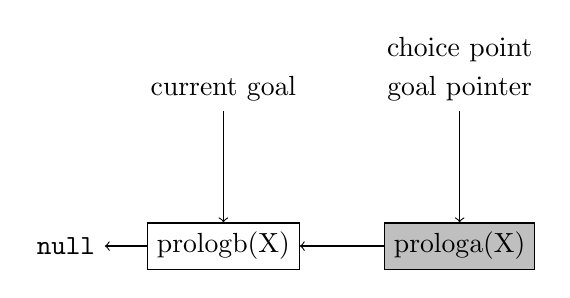
\begin{tikzpicture}[box/.style={draw, rectangle}]
  \node[box] (B) at (0, 0) {\mintinline{prolog}{b(X)}};
  \node[box, fill=lightgray] (A) at (3, 0) {\mintinline{prolog}{a(X)}};

  \node (null) at (-2, 0) {\texttt{null}};
  \node (current) at (0, 2) {current goal};
  \node (cp1) at (3, 2.5) {choice point};
  \node (cp2) at (3, 2) {goal pointer};

  \draw[->] (A) -- (B);
  \draw[->] (B) -- (null);
  \draw[->] (current) -- (B);
  \draw[->] (cp2) -- (A);
\end{tikzpicture}
\vspace{5mm}
\caption{The goal graph after the first resolution}
\end{subfigure}
\vspace*{-5mm}
\caption{The goal graph}
\label{fig:goals}
\end{figure}

Figure \ref{fig:goals} illustrates this idea. Before resolving \mintinline{prolog}{a(X)} with \mintinline{prolog}{a(1)} (c), a choice point is created, containing a pointer to the current goal. After the resolution step, \mintinline{prolog}{a(X)} is ``popped from the goal stack'', which is implemented by setting the current goal pointer to its predecessor (d). Importantly, however, it remains in the graph, as upon backtracking to the choice point when \mintinline{prolog}{b(1)} fails, the current goal pointer is restored to that stored in the choice point. In order to prevent the goal stack growing indefinitely, each choice point also contains the number of goals in the stack when it was created, and the goal stack is truncated to this size upon backtracking. The goal stack is also garbage collected (Section \ref{sec:gc-impl}).

\paragraph{Code Area} There is no separate code area, as the clauses of the program are stored on the heap using the same representation as regular terms, an idea suggested by Tarau \cite{tarauHitchhikersGuideReinventing2018}. Initially, my implementation did use a distinct code area with a different representation, but profiling revealed that, in the former implementation, up to 40\% of the execution time was spent copying terms onto the heap. Benchmarking confirmed that Tarau's approach reduced execution time by around 25\% across various benchmarks (Section \ref{sec:benchmarking}).

In this implementation, copying a clause onto the heap when a goal unifies with its head consists of a single \texttt{memcpy} followed by a linear scan of the copied clause terms to add the appropriate offset to any pointers. To efficiently identify the byte boundaries between terms in the body of the clause, each clause additionally includes a ``header'' containing $n$ variables, bound to each of the $n$ terms in its body.

\subsection{Pointers}

A common theme in the implementation of this project, taken from WebAssembly, is that of using indexing over pointers. The contiguous nature of the heap allows terms to be referred to by their index, and the same is true for the goal stack and choice point stack.

Rust strongly discourages the use of raw pointers, instead preferring its memory-safe abstraction, references. Every object in Rust must have exactly one \emph{owner}, with multiple immutable references or a single mutable reference allowed, enforced at compile time by the \emph{borrow checker}. The Prolog heap does not fit nicely into this model: there may be multiple variables bound to the same term, both of which requiring mutable access to it (e.g. to update the term when unifying). One way to work around this is to use reference counting and \texttt{RefCell}, which facilitates runtime borrow checking, but this is very expensive in terms of performance. Instead, terms are referred to by their index in the heap. As we use a merged heap/stack architecture, this is straightforward to implement. Hereafter, any references to ``pointers to heap terms'' actually mean indices.

The performance consequences of these approaches are discussed in more detail in Section \ref{sec:get-unchecked}.

\subsection{Term Representation}

Terms are stored on the heap as fixed-size blocks of 24 bytes. In Rust, these are represented as an enum (Figure \ref{fig:rust-term-representation}), Rust's sum type.

Atoms are typed, being either strings, integers, or floats, with implicit casting from integers to floats permitted. The representation of variables includes a pointer to their bound object, as in the WAM, but additionally a boolean flag to indicate whether they are \emph{shunted} (Section \ref{sec:variable-shunting}), which is used in garbage collection. Compound terms, represented by their functor and arity $n$, are followed in the heap by $n$ variables pointing to each of their arguments. There is also a heap representation of cut, which is necessary because goals are stored on the heap. Finally, \emph{lambda terms}, used to call JavaScript code from within the Prolog execution (Section \ref{sec:js-ffi}), are represented in the same way as compound terms, except instead of storing a functor, they store the raw JavaScript code.

All other kinds of term supported in the Prolog syntax are syntactic sugar for terms represented as above, converted during parsing. For example, the arithmetic expression $2 + 3$ becomes the compound term \texttt{+(2, 3)}, and the list \texttt{[a, b]} becomes the compound term \texttt{.(a, .(b, []))}.

\begin{figure}[H]
\centering
\begin{subfigure}{0.5\textwidth}
\centering
\begin{minted}{rust}
pub enum HeapTerm {
    Atom(Atom),
    Var(HeapTermPtr, bool),
    Compound(StringId, usize),
    Cut(ChoicePointIdx),
    Lambda(StringId, usize),
}
\end{minted}
\end{subfigure}%
\begin{subfigure}{0.5\textwidth}
\centering
\begin{minted}{rust}
pub enum Atom {
    String(StringId),
    Integer(i64),
    Float(f64),
}


\end{minted}
\end{subfigure}
\caption{Term representation in Rust}
\label{fig:rust-term-representation}
\end{figure}

\subsection{Parsing}

The Prolog program is parsed into its abstract syntax tree (AST) using a parser generated by LALRPOP \cite{thelalrpopprojectdevelopersLALRPOPhttpsgithubcom2015} with a custom grammar, written from scratch.

\begin{figure}[H]
\centering
\begin{minted}{rust}
Clause: Clause = {
    <h:Term> "." => Clause(h, vec![]),
    <h:Term> ":-" <b:Comma<Term>> "." => Clause(h, b),
}
Comma<T>: Vec<T> = {
    <t:T> => vec![t],
    <mut ts:Comma<T>> "," <t:T> => { ts.push(t); ts },
}
\end{minted}
\caption{Extract from the LALRPOP grammar}
\label{fig:grammar}
\end{figure}

Figure \ref{fig:grammar} shows an extract from the grammar. LALRPOP supports polymorphic non-terminals, which are used in the extract to define a generic non-empty comma-separated list of terms, \texttt{Comma<T>}. The \texttt{vec!} macro is used to create a vector using array-like syntax.

\subsection{Built-in Predicates}

\label{sec:builtins}

In order to do useful computation, the interpreter must support a set of built-in predicates, such as arithmetic evaluation. The full list of built-in predicates is given in Appendix \ref{appendix:predicates}.

Each predicate implements a \emph{trait} called \texttt{Builtin}, which is similar to an interface in C++ or Java. The definition of this trait is shown in Figure \ref{fig:builtin-trait}. This trait has an associated constant, \texttt{ARITY}, which is the number of arguments the predicate takes. A pointer to the first argument is passed to the \texttt{eval} function. This function evaluates the predicate, potentially modifying the state of the interpreter through the mutable reference to the \texttt{Solver} object, returning a boolean if the predicate succeeded or failed with no errors, or an error otherwise, for example if an argument was insufficiently instantiated.

\begin{figure}[H]
\centering
\begin{minted}{rust}
pub trait Builtin<const ARITY: usize> {
    fn eval(solver: &mut Solver, args: HeapTermPtr)
        -> Result<bool, BuiltinError>;
}
\end{minted}
\caption{The \texttt{Builtin} trait}
\label{fig:builtin-trait}
\end{figure}

Many built-in predicates are implemented almost identically, for example the extra-logical type testing predicates \texttt{var/1}, \texttt{atom/1}, and \texttt{integer/1} (among others), which only differ in the type they compare against. To avoid code duplication, these predicates are implemented using meta-programming, with a \emph{macro} generating the code for each type. Figure \ref{fig:builtin-macro} shows the macro for type testing predicates. It uses Rust's pattern matching syntax to match the heap representation of the term against a pattern \texttt{\$matcher} representing the type to check for.

\begin{figure}[H]
\centering
\begin{minted}{rust}
macro_rules! impl_type_check {
    ($name:ident, $matcher:pat) => {
        pub struct $name;
        impl Builtin<1> for $name {
            fn eval(solver: &mut Solver, args: HeapTermPtr)
                -> Result<bool, BuiltinError>
            {
                Ok(matches!(solver.heap.get(args), $matcher))
            }
        }
    };
}

impl_type_check!(IsIntegerBuiltin, HeapTerm::Atom(Atom::Integer(_)));
impl_type_check!(IsAtomBuiltin, HeapTerm::Atom(_));
impl_type_check!(IsVarBuiltin, HeapTerm::Var(_, _));
\end{minted}
\caption{Macro for type testing predicates}
\label{fig:builtin-macro}
\end{figure}

\subsection{Cut}

The cut operator, \texttt{!/0}, is an extra-logical predicate that commits to the clause in which it appears. In other words, backtracking past a cut causes the clause it appears in to fail.

When a clause is copied onto the heap, a linear scan updates its variables by the appropriate offset (Section \ref{sec:memory-layout}). This linear scan also updates the heap representations of any instances of the cut operator to include the index of the current choice point, that is, the choice point before this clause was selected. When the cut operator becomes the current goal, the choice point stack is truncated to the choice point it refers to.

\subsection{Choice Point Elimination (incl. Last Call Optimisation)}

Last call optimisation (LCO) is traditionally implemented by reusing the stack frame for the last call of a determinate predicate (Section \ref{sec:preparation-implementation}). This is only applicable on the final clause of a predicate, as otherwise the predicate would not be determinate.

However, in my implementation, we do not have a call stack, instead storing all terms on the heap and using a goal stack and choice point stack for control (Section \ref{sec:memory-layout}). Therefore, LCO must be implemented in two parts, one on the choice point stack and one on the goal stack.

For the choice point stack, I implement a variant of last call optimisation, which I call \emph{choice point elimination}. This works by not creating a choice point for the final clause of a predicate, as its failure necessarily implies the failure of the entire predicate. Static analysis prior to execution is performed to group clauses into predicates to enable this optimisation. This has the same effect as traditional LCO: if a clause is determinate, it will not leave any choice points on the stack, as no choice point will be created for either the choice of the clause or the solution of any goals.

Recall the implementation of the goal stack from Section \ref{sec:memory-layout}, namely that ``popping a goal from the stack'' does not remove it from the graph, rather moving the current goal pointer to its predecessor. Goals are only fully removed on backtracking, when the goal stack is truncated to the size it was when the choice point was created. As is, while a determinate predicate will use constant space on the choice point stack, it will use linear space on the goal stack.

However, when no choice points refer to a goal, it is sound to remove it from the graph entirely when it is popped. This is exactly the case in a determinate predicate. The goals of its body are pushed to the goal stack when a goal unifies with its head, and because of its determinacy and choice point elimination, no choice points are created as these goals are popped and resolved one by one. Furthermore, as they will be allocated at the end of the memory for the goal graph, no fragmentation occurs when they are removed. This is implemented by passing a boolean flag to the \texttt{Goal::pop} function, indicating whether the goal can be safely removed from the graph (Figure \ref{fig:goal-pop}).

\begin{figure}[H]
\centering
\begin{minted}{rust}
impl Goal {
    pub fn pop(&mut self, determinate: bool) {
        if let Some(ptr) = self.current.take() {
            self.current = self.goals[ptr].prev_ptr();
            if determinate && ptr == self.goals.len() - 1 {
                self.goals.pop();
            }
        }
    }
}
\end{minted}
\caption{Implementation of \texttt{Goal::pop}}
\label{fig:goal-pop}
\end{figure}

\subsection{String Interning}

Strings are expensive to copy because they must be dynamically allocated in the linear memory. Comparing two strings for equality is also orders of magnitude more expensive than a simple arithmetic comparison, requiring both memory reads and $O(n)$ comparisons (where $n$ is the length of the string), as opposed to a single WebAssembly instruction for arithmetic comparison.

For this reason, the implementation avoids using \texttt{String} objects wherever possible by using \emph{string interning}. All strings are allocated in a specific area of memory, and all references to each string are replaced with its index in that area. A hash table, mapping strings to their indices, is used to ensure that no duplicate strings appear.

A further optimisation initialises the string area with fixed mappings for commonly-used strings, such as the names of built-in predicates and arithmetic operators. For example, the string \texttt{"+"} is always at index 9, stored as a constant \texttt{str::ADD} in the Rust code, so a real string comparison is not necessary, even with runtime-generated strings (due to the uniqueness of string mapping). Figure \ref{fig:fixed-string-indices} shows how this is used in the arithmetic evaluation code (simplified).

\begin{figure}[H]
\centering
\begin{subfigure}{.5\textwidth}
\centering
\begin{minted}{rust}
match functor {
    str::ADD /*  9 */ => add(&a, &b),
    str::SUB /* 10 */ => sub(&a, &b),
    str::MUL /* 11 */ => mul(&a, &b),
    str::DIV /* 12 */ => div(&a, &b),
    ...
}
\end{minted}
\caption{Arithmetic comparison of functors}
\end{subfigure}%
\begin{subfigure}{.5\textwidth}
\centering
\begin{minted}{rust}
match functor {
    "+" => add(&a, &b),
    "-" => sub(&a, &b),
    "*" => mul(&a, &b),
    "/" => div(&a, &b),
    ...
}
\end{minted}
\caption{String comparison of functors}
\end{subfigure}
\caption{Using fixed string indices for arithmetic evaluation}
\label{fig:fixed-string-indices}
\end{figure}

\section{Garbage Collection}

\label{sec:gc-impl}

Garbage collection is a crucial part of a merged heap/stack architecture \cite{liEfficientMemoryManagement2000}. This section describes the implementation of the garbage collector in the Prolog interpreter.

\subsection{Mark and Sweep}

Initially, I implemented a naive mark-and-sweep garbage collector, based on the algorithm described by Knuth \cite{knuthArtComputerProgramming1997}.

The mark phase uses the goal stack, choice point stack, and named variables in the query as the root set, marking all terms on the heap that are reachable from these roots. A term is marked by setting its entry in a separate vector called the \emph{garbage collection map} (Knuth calls these entries \texttt{LINK}s) to \texttt{GC\_MARKED}. The entries are initialised to \texttt{GC\_UNMARKED} at the start of each garbage collection.

During the compaction phase, a linear scan of the heap is performed, shuffling marked terms down the heap to remove gaps. The heap is then truncated to the end of the last marked term. The garbage collection map is also updated to reflect the new locations of terms.

Finally, during the pointer rewriting phase, the heap is scanned again, and all pointers are updated using the garbage collection map. Pointers in the root set are similarly updated.

\subsection{Precise Garbage Collection}

The key aim of this part of the project was to implement a \emph{precise} garbage collector, as defined by Wielemaker and Neumerkel in their paper evaluating the garbage collectors of various Prolog implementations \cite{wielemakerPreciseGarbageCollection2008}:

\begin{quote}
``We define a `precise' garbage collector as a garbage collector that reclaims all data that can no longer be reached considering all possible execution paths from the current state without considering semantics.''
\end{quote}

They define five programs that must run indefinitely in bounded memory with a precise garbage collector. Two of these concern functionality not relevant to this project, regarding attributed variables and if/then/else constructs. The remaining three are shown in Figure \ref{fig:gc-programs}.

\begin{figure}[H]
\centering
\begin{subfigure}{.65\textwidth}
\centering
\begin{minted}{prolog}
run :- run(_,_).
run(L0, L) :- f(L0, L1), dummy(L1, L).
f([g|X], Y) :- f(X, Y).
dummy(Xs, Xs).
\end{minted}
\caption{And-control (head variables)}
\end{subfigure}%
\begin{subfigure}{.35\textwidth}
\centering
\begin{minted}{prolog}
run :- run(_).
run(X) :- f(X).
run(X) :- X == [].
f([f|X]) :- f(X).
\end{minted}
\caption{Or-control}
\label{fig:or-control}
\end{subfigure}
\par\bigskip
\par\bigskip
\begin{subfigure}{\textwidth}
\centering
\begin{minted}{prolog}
run :- run(_,_).
run(L0, L) :- dummy(L0, L1), f(L1, L2), dummy(L2, L).
f([f|X], Y) :- f(X, Y).
dummy(Xs, Xs).
\end{minted}
\caption{And-control (existential variables)}
\end{subfigure}
\caption{Garbage collection test programs}
\label{fig:gc-programs}
\end{figure}

In order to meet these criteria, a number of Prolog-specific garbage collection optimisations were made. These are described in the following sections.

\subsection{Variable Shunting}

\label{sec:variable-shunting}

\emph{Variable shunting} replaces variables that are only seen in their bound state with their binding values \cite{sahlinVariableShuntingWAM1991}. These variables are those which were created and then bound without the creation of any choice points in between. I implement variable shunting using the ``timestamping'' algorithm described by Bekkers et al. \cite{bekkersDynamicMemoryManagement1992}.

Figure \ref{fig:shunt-program} shows a program that demonstrates the need for variable shunting. Y can be shunted to prevent the heap from growing indefinitely.

\begin{figure}[H]
\centering
\begin{minted}{prolog}
f(X) :- Y = X, f(Y).
?- f(3).
\end{minted}
\caption{A program that demonstrates the need for variable shunting}
\label{fig:shunt-program}
\end{figure}

Bekkers et al. define the \emph{age} of a variable to be the serial number of the choice point created just after that variable, i.e. the number of choice points on the stack when the variable was created. In the merged heap/stack architecture, due to the chronological layout of the heap, it is equivalent, and simplifies the implementation, to consider the age of a variable to be simply its index in the heap. The age of a choice point is defined to be the size of the heap when it was created.

The timestamping algorithm works in two parts, the first during unification and the second during garbage collection, between the mark and compact phases.

\begin{enumerate}
\item Prior to unifying a variable with another term, the age of the variable is compared to the age of the current choice point. If the variable is older, it is pushed to the trail as normal. Otherwise, no choice points can exist since its creation, so variable shunting is applicable. The variable is not pushed to the trail and is instead marked as shunted by setting a flag in its heap representation. This is shown in Figure \ref{fig:unify-var}.

\begin{figure}[H]
\centering
\begin{minted}{rust}
#[inline]
fn unify_var(&mut self, a: HeapTermPtr, b: HeapTermPtr) -> bool {
    if a < self.choice_point_age.0 {
        self.trail.push(a);
    } else {
        self.heap.mark_shunted(a);
    }

    self.heap.unify(a, b);
    true
}
\end{minted}
\caption{Variable shunting during unification}
\label{fig:unify-var}
\end{figure}

\item During garbage collection, an additional ``shunt'' phase is added between the mark and compact phases. The shunt phase iterates over the heap, from younger to older terms (reverse order), and for each shunted variable that was marked, performs one of two actions, based on the garbage collection map entry of the term it is bound to:
\begin{enumerate}
\item If the term is not yet mapped, the variable is mapped to the term.
\item If the term is mapped to an index $i$, it must be a younger variable that has already been shunted by case (a). Therefore, the variable is also mapped to $i$.
\end{enumerate}

These cases are illustrated in Figure \ref{fig:shunt-cases}. The following compact phase then considers all terms that were already mapped by the shunt phase to be dead, and reclaims them. It also performs a final pass over the map to update the entries of all shunted variables to point to their new (post-compaction) locations.

\begin{figure}[H]
\centering
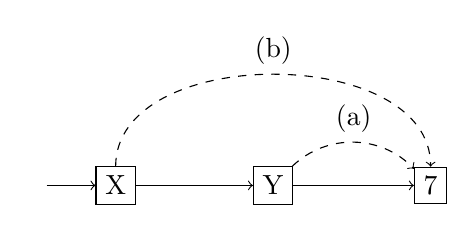
\begin{tikzpicture}[box/.style={draw, rectangle}]
    \node (root) at (-1, 0) {};
    \node[box] (X) at (0, 0) {X};
    \node[box] (Y) at (2, 0) {Y};
    \node[box] (7) at (4, 0) {7};

    \draw[->] (root) -- (X);
    \draw[->] (X) -- (Y);
    \draw[->] (Y) -- (7);

    \draw[->, dashed] (X) to [bend left=90] node [midway, above] {(b)} (7);
    \draw[->, dashed] (Y) to [bend left=45] node [midway, above] {(a)} (7);
\end{tikzpicture}
\caption{Variable shunting during garbage collection. X and Y are shunted variables. Solid lines represent variable bindings, and dashed lines represent the garbage collection map.}
\label{fig:shunt-cases}
\end{figure}

\end{enumerate}

\subsection{Early Reset}

\emph{Early reset} is concerned with collecting terms that are only accessible from a choice point \cite{applebyGarbargecollectionProlog1988}.

Recall the program in Figure \ref{fig:or-control} (or-control). The first clause of \texttt{run/1} creates a choice point to try the second clause if the first fails, then iterates through an infinite list. As is, the garbage collector is prevented from reclaiming items already iterated over because they are still reachable from the choice point: in the goal \texttt{run(X)}, \texttt{X} is bound to the infinitely-growing list by the execution of the first clause. The key insight behind early reset is that \texttt{X} will be unbound upon backtracking, before the second clause is reached, so it is safe to reset it if it is only reachable from the choice point.

This is implemented during the mark phase. The root set is ordered such that marking from the choice point stack is done last, so that terms only reachable from the choice point stack can be identified. The trail stack is then scanned from the point of each choice point to the end, and any variables that are currently unmarked (i.e. only reachable from the choice point stack, if at all) are reset.

\subsection{Testing for Precise Garbage Collection}

Variable shunting and early reset prove sufficient to meet the criteria for precise garbage collection.

To test this, for each of the programs in Figure \ref{fig:gc-programs}, I use the following algorithm:

\begin{enumerate}
\item Run the program for a fixed number of iterations to reach a steady state.
\item Perform a garbage collection, then measure the size of the heap.
\item Run the program for a further fixed number of iterations.
\item Perform a garbage collection and measure the size of the heap, passing the test if the heap size is less than or equal to that in step 2.
\item Make one resolution step, then go back to step 4. Repeat this a fixed number of times in order to get to the same point in the execution as the first measurement, at which point the test passes.
\end{enumerate}

\subsection{Generational Garbage Collection}

\label{sec:implementation-generational-gc}

While the naive mark-and-sweep garbage collector augmented with variable shunting and early reset is precise, it is not particularly efficient.

Generational garbage collection avoids scanning the entire heap by dividing it into generations, with the youngest generation being collected most frequently (Section \ref{sec:generational-gc}).

\emph{Segmented garbage collection} applies this concept to Prolog \cite{applebyGarbargecollectionProlog1988}. Recall the concept of \emph{age} from the variable shunting algorithm (Section \ref{sec:variable-shunting}). This is used to divide the heap into generations, where each generation consists of a choice point and all terms not older than it, up to the next choice point. When a choice point (and hence a new generation) is created, all non-garbage terms in previous generations cannot become garbage until the choice point is popped upon backtracking. This means that each garbage collection needs only consider terms in generations for which garbage collection has not yet been performed.

This is implemented by keeping track of the age of the oldest choice point for which garbage collection has not yet been performed. Initially, this is set to 0. When a garbage collection is performed, the age is updated to the age of the current choice point. When a choice point is popped, the age is updated to the age of the choice point before it.

\section{JavaScript FFI}

\label{sec:js-ffi}

\section{Web-Based Development Environment}